\documentclass[12pt,a4paper]{article}
\addtolength{\textheight}{2.6cm}

\usepackage[utf8]{inputenc}
\usepackage[T1]{fontenc}
%\usepackage[english,swedish]{babel}
\usepackage{amsmath}
\usepackage{ae}
\usepackage{color}
\usepackage{graphicx}
\usepackage{caption}
\usepackage{subcaption}
\usepackage{verbatim}
\usepackage[backend=bibtex,
style=numeric
%style=alphabetic
%style=reading
]{biblatex}
\addbibresource{Library}
\newcommand{\N}{\ensuremath{\mathbbm{N}}}
\newcommand{\Z}{\ensuremath{\mathbbm{Z}}}
\newcommand{\Q}{\ensuremath{\mathbbm{Q}}}
\newcommand{\R}{\ensuremath{\mathbbm{R}}}
\newcommand{\C}{\ensuremath{\mathbbm{C}}}
\newcommand{\rd}{\ensuremath{\mathrm{d}}}
\newcommand{\id}{\ensuremath{\,\rd}}

\begin{document}

\author{DAT300 \\\\
Johannes Blomquist johblom@student.chalmers.se \\
Anders Nordin anordin@student.chalmers.se \\
}
\title{\textsc{Home automation system for handling peaks in the power consumption}}
\date{\today}

\clearpage\maketitle
\thispagestyle{empty}
\newpage

\thispagestyle{empty}
\begin{abstract}
Global warming is an acknowledged threat \cite{root2003fingerprints}. To lower the average temperature we must minimize the emission of greenhouse gases. One might argue that the obvious solution is to consume less energy. However, it is also possible to achieve the same result by, instead of lowering the consumption, redistribute it in an efficient manner such that people do not need to change their behaviour. This statement originates from the problem with power consumption peaks that occur in the electrical grid when people perform their daily routines at the same time. The power suppliers need to produce, at minimum, the requested amount of power. Adaption to such energy consumption peaks in the grid is also very expensive for the power suppliers. In this project we demonstrate that it is actually possible to minimize the peaks by using algorithms that schedule different electrical equipment in a household more efficiently. Based on previous research we demonstrate, on a small scale, how private customers can help to flatten peaks with respect to other customers and the grid. We evaluate our results in a testbed where we control electrical devices with the help of smart-plugs, where the algorithms is implemented in Python. We compare our approach with similar solutions, and discuss strengths and weaknesses, as well as possible improvements.
%% Korrekturläst av Anders 2014-12-02

\end{abstract}
\newpage
\clearpage
\tableofcontents
%\listoffigures
\newpage

\pagenumbering{arabic}
\setcounter{page}{1}
\section{Introduction}
We have seen an increased number of products on the market which are equipped with the ability to communicate and monitor its power consumption, an example of this is the \emph{Samsung WW9000 washing machine} \cite{samsungww9000}. Smart devices are typically off-the-shelf products that can both be used to ease everyday life but also to lower their power consumption. Another similar product, \emph{100Koll}, is provided by the energy provider E.ON \emph{100Koll}. \emph{100Koll} lets you keep track of the household's total consumption and also, with the help of smart plugs, keep track of certain devices. The service can also help you keep a monthly budget for the power consumption as well as the ability to shut off devices remotely from a smart phone application \cite{eon}.

Our work, summarized in this report, aims to show a practical example of a system that schedules home appliances in order to lower power peaks. The work is based on the article \emph{Smartcap: Flattening peak electricity demand in smart homes by Barker et al.} \cite{barker2012smartcap}. The system will be tested with data from a real home in order to compare it against the same data without the system.

Besides the practical part we also evaluate the scheduler and suggest improvements as future work. The report also consists of a part with other solutions to the problem.

The report is structured as follows. This section gives an introduction to the reader with background and the actual problem, section \ref{sec:related work} discusses similar approaches, section \ref{sec:implementation} describes the implementation of the project, section \ref{sec:discussion} evaluates the result and discusses flaws. Finally, in section \ref{sec:conclusion} we summarize the project and propose future work.

\subsection{Background and Problem Formulation}
People tend to have similar daily routines; they wake up approximately at the same time, cook breakfast and then go to work. Figure \ref{peakconsumption} illustrates the consumption trace for one household during a day where daily routines are clearly distinguished. When a whole neighbourhood starts cooking their breakfast at the same time, the peaks would be even more extreme. Therefore, the residential distribution network suffers high peaks in the power demand during meal hours and evenings, sometimes as much as ten times higher demand than during nights or when there is nobody at home. Since there is normally no local storage in the power grid, the energy provider needs at all time to produce roughly as much electricity that is being consumed. That means, for example, we may have full electricity production during lunchtime, but one hour later that could be dropped to half that amount. 

Numbers from 2008 state that households account for 40 \% of the total electricity usage in Sweden \cite{WNA}. The power is generated from different sources. Nuclear and hydro power represents the base load. During production, both nuclear and hydro power is relatively cheap and their emission of greenhouse gases is very small \cite{WNA}. However, when the demand for electricity peaks electricity providers need to produce more power or else a power outage would occur. This additional part comes from reserves which can respond quickly to the changing demand, so-called spinning reserves. Spinning reserves often consists of gas turbines. However, burning gas is not environmentally friendly and is also quite expensive to use \cite{svenskenergi}. If the load was more regular, without the peaks, a much more even and lower electricity production could be used, which would in turn yield a lower cost and less emission of greenhouse gases.

\begin{figure}[!h]
\centering
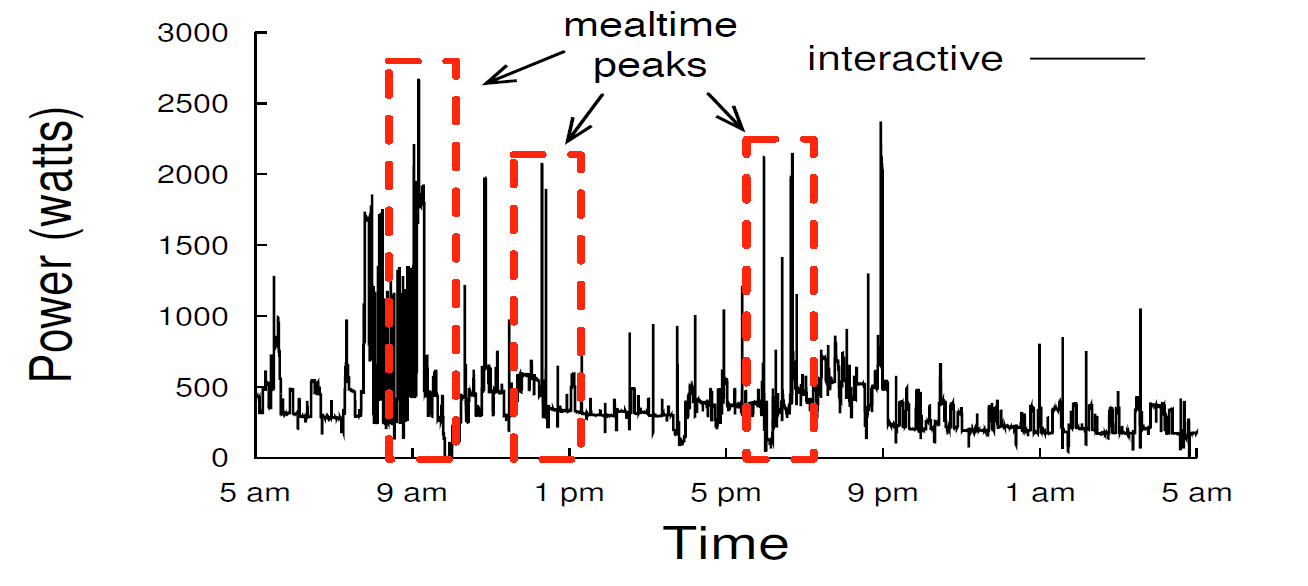
\includegraphics[width=1.0\textwidth]{img/peakdemand.png}
\caption[Peaks]{\emph{\small Power consumption in a household, meal time peaks highlighted \cite{barker2012smartcap}}}
\label{peakconsumption}
\end{figure}
 
We define two types of residential loads. The first one is referred to as background load. It consists of devices which are constantly plugged in, but does not always consume power, e.g. fridge, air condition and floor heating. The power units in these devices are only activated when the measured value from the environment(e.g. temperature) differs too much from the set value.

The second term is called the interactive load and consists of devices such as microwave, radio and TV. These devices are much harder to predict since people activate them when they need to use them. It is not possible to control the interactive load without interfering with the living habits of the residents. It should be pointed out that one goal of our work aims is to demonstrate a solution which do not disturb the residents of the house. We describe the solution in section \ref{sec:implementation}.

\subsection{Limitations}
The system is built in a small scale with limited test data to show the concept. The model will hold a couple of devices connected and monitored to test and validate the solution. We evaluate one of several possible solutions to the problem. Further solutions will be discussed in section \ref{sec:discussion}.

The data set we use for testing consists of 24 hours of data from a single household. We are aware of the limited test data and therefore we suggest that the algorithm should be tested more extensively by including more homes over a longer period to the test data.
%% Korrekturläst av Anders 2014-12-03

\newpage
\section{Related Work}
\label{sec:related work}
There has been previous research in the area of peak demand. Johnson et al. propose a system where a battery should be placed between the electricity provider's distribution grid and the customer's home \cite{johnson2011energy}. The system operates in three different modes, depending on thresholds. The system could request the household's exact electricity demand at that time. It could also request more than the demand and use the excessive electricity to charge the battery. Finally, it could request less than the current demand and fill the gap with electricity from the battery. The idea with this concept is to charge the battery whenever the household is idle and then use power from the battery when there is more activity, e.g. when cooking dinner \cite{johnson2011energy}.

The proposed method is indeed an interesting one, but it also has its difficulties. One problem is to determine how large the battery should be. The battery accounts for a significant part of the system's initial cost, a large battery is more expensive than a smaller one. On the other hand, a battery that is relatively big could result in a completely flat demand curve. Furthermore, in-depth knowledge of the prospected household's demand curve is needed to calculate the size of the battery since this varies from household to household. The goal is to find the smallest battery that can achieve the optimal peak demand. Another battery related problem is that batteries suffer from energy losses when transforming alternating current (used in the power grid and outlets) to direct current (used to store electricity in the battery). This means that the bigger the battery is, the bigger the loss is. Furthermore, today's batteries have a limited charge and discharge cycle, i.e. they lose charging capability when they are used and therefore need to be replaced after some time. This is also an incentive to choose the battery size with care. Johnson et al. also points out another issue to resolve. Since it is very hard to anticipate the future, i.e. the power demand for the next hour, it is very problematic to find efficient charge and discharge algorithms. A system that makes bad decisions about when to charge and discharge the battery is even likely to perform worse then if the system was removed. The complicated part is finding an algorithm that is not too greedy, i.e. an algorithm that does not react too fast when small changes occur in the demand curve. A greedy algorithm would simply alternate between charge and discharge for every little peak and trough in the demand. On the other hand, if the algorithm is more generous it might be too focused on lowering the maximum peak that it does not consider all other peaks that occur during a day.

Georgiadis and Papatriantafilou \cite{georgiadis2013greedy} propose a model for the problem of unforecasted energy dispatch and storage, where electric vehicles are mentioned as possible energy storage. Furthermore, a greedy online algorithm that dispatches the load and utilizes storage capabilities efficiently is suggested. 

Gaing \cite{gaing} also proposes a solution to the dispatch problem, but with focus on the economic aspects. Gaing uses a particle swarm optimization heuristic method for solving the economic dispatch in power system.

\newpage
\section{Implementation}
\label{sec:implementation}
The prototype is tailored to a smaller scale of a home environment. It has features to control and monitor the power consumption from each device included in the background load, which, in our data set, corresponds to a fridge and a floor heater. We also gain data from the total power consumption, where interactive load is included. The implemented and evaluated algorithm to the problem with peak avoidance is based on the one found in \cite{barker2012smartcap}.

\subsection{Test Data}
At this stage we do not have a real home environment to run our system in and we have therefore acquired 24 hours of test data from a real home in Sweden and fed it to our system through an \emph{SQLite} database. Since the behaviour of the background loads will be altered in our system, their normal behaviour must be analyzed in order to estimate how long the respective load can be powered down before they must be powered up again and vice versa. 

In figure \ref{PowerTrace} the consumption trace of the fridge and the floor heater from the database is illustrated. Since the test data is not that fine grained (10 minutes interval) the analysis of the behaviour is only approximate. It is concluded that this fridge, which typically operates in temperatures between four to six degrees, can be powered down for approximately 20 minutes before the temperature reaches the upper bound if it begins at the lowest temperature. It then needs to be powered for 80 minutes before reaching the lower bound again. When powered, the fridge consumes about 16 watts in average. It should also be noted that if the fridge door is opened, the temperature will rise much faster and the fridge will need power sooner than predicted. This phenomenon however, has not been clearly noticed in the test data from the fridge and is therefore neglected in our simulation, but would automatically be taken into account in a real-life scenario.

The floor heater can have much longer down time. It can be powered down for 30 minutes before the temperature reaches its lower bound and then needs to be powered for 10 minutes. Thus, the floor heater also requires much less on-time than the fridge, but on the other hand, the consumption of the floor heater, when powered up, is 80 watts during most hours, but with a severe peak in the afternoon with a consumption of a staggering 180 watts. There are a few possible explanations for this peak. It could be that the floor heater is on a timer that will increase the temperature just before the occupants get back home from work. It could also be that the occupants get home on a winter day and brings snow inside. The temperature on the floor will then drop and extra power is needed to satisfy the set temperature bounds. The reason is not important, but the extra consumption of the floor heater during certain hours is considered in our scheduler.


\begin{figure}[!h]
\centering
    \begin{subfigure}[b]{0.52\textwidth}
            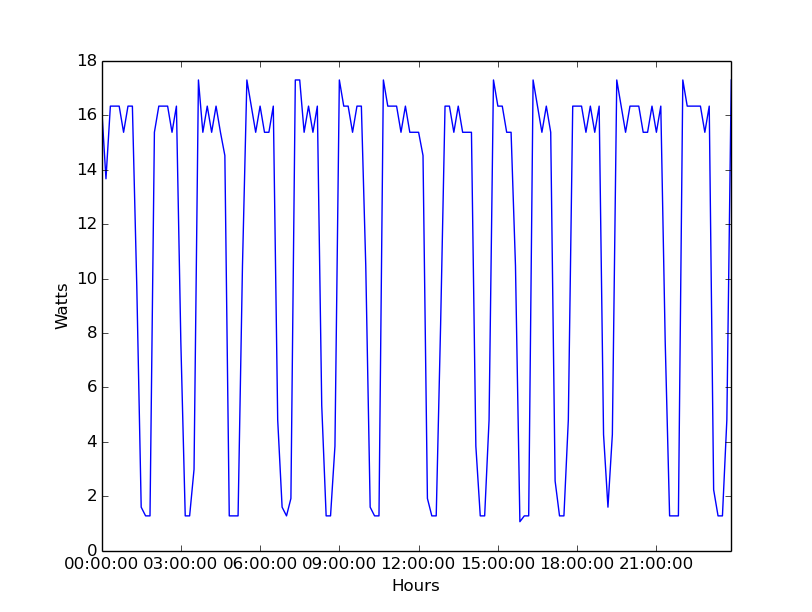
\includegraphics[width=\textwidth]{img/fridge.png}
            \caption[Peaks]{\emph{\small Fridge.}}
            \label{fig:fridgePowerTrace}
        \end{subfigure}%
        ~
        \begin{subfigure}[b]{0.52\textwidth}
            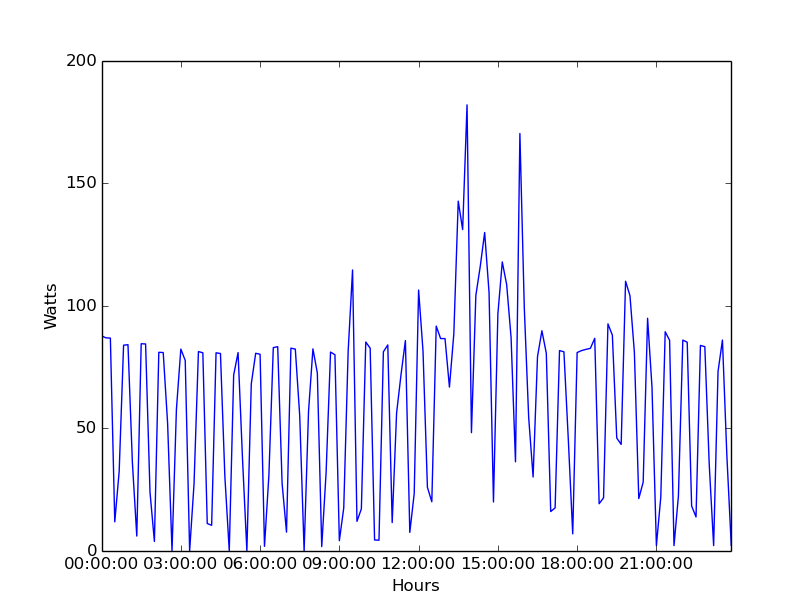
\includegraphics[width=\textwidth]{img/floor_heating.png}
            \caption[Peaks]{\emph{\small Floor heater.}}
            \label{fig:floorHeaterPowerTrace}
        \end{subfigure}%
\caption[Peaks]{\emph{\small Consumption trace of background loads.}}
\label{PowerTrace}
\end{figure}

\subsection{Least Slack First (LSF)}

Likewise the article by Baker et al. we use the \emph{Least Slack First} (LSF) algorithm to schedule devices that represent the background load. It should be noted that the LSF algorithm is inspired by the well known earliest deadline first algorithm used in real-time operating systems \cite{barker2012smartcap}. 

In the algorithm there is a consumption threshold that ensures we do not power up too many appliances at the same time. The algorithm sums the total consumption of all active interactive loads and then power background loads until the total load crosses the threshold. The threshold, in our solution, is a calculated average of the last hour's consumption. Choosing such an average will make the threshold follow the natural shift in power demand during different hours of the day. If some background load has slack zero it will, if necessary, breach the threshold since this load must have power. The difference between our solution and the one presented by Barker et al. is that we also consider the interactive loads when calculating the threshold and when scheduling the background loads. This means that our solution could take action and power down all background loads if there is a high peak in the interactive loads in order to prevent the highest peaks. 

For the solution to be attractive and possible to implement in homes, it must not require a change of habits of the occupants. Therefore, all bounds discussed in the previous section must be held and no interactive load can be controlled from the system. In this report we define slack as the measure of how long a background load can remain off without affecting its bound, e.g. the temperature in the fridge. The device that has the least slack will have priority over the others. If the slack reaches zero for some device, the device is forced to start, no matter what the current load from other devices is.

\subsection{System Description}
The system consists of a scheduler developed in Python. The scheduler in turn communicates with an \emph{SQLite} database which holds test data for a 24-hour period. The nodes are built with the help of an off-the-shelf system called \emph{Plugwise} \cite{plugwise2014}. \emph{Plugwise} handles the communication between devices in the home using a wireless \emph{Zigbee} meshed network. Since \emph{Plugwise} does not offer any open API we have used a third-party library to communicate with the nodes \cite{hadaraplugwise}. The hardware we used belong to the product \emph{Plugwise} and consists of two power switches, which are controlled from our computer by a USB wireless adapter.

The prototype consists of one coordinator thread and then one thread for each background load. The background threads monitor the slack of each device and also turn the power to the device on and off. The coordinator thread monitors the current consumption from the interactive loads and together with the reported slack from the background threads makes the scheduling decisions and orders the background threads to power their device on or off.

While running the simulation we plot the result dynamically, showing the difference in real-time. In figure \ref{runView} we illustrate our system. In the picture we have a fridge and an air conditioner (in the simulation the AC is replaced with a floor heater). We also have a third variable, the interactive loads (television, radio, computer, coffee maker), which will affect the other two when started, but cannot be controlled by the system.

\begin{figure}[!ht]
\centering
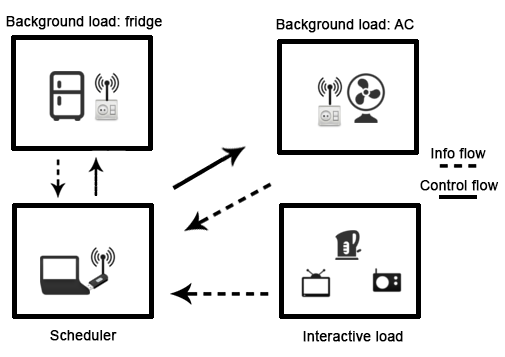
\includegraphics[width=0.75\textwidth]{img/dat300_final_desc.png}
\caption[Project Description]{\emph{\small Description of the implemented system.}}
\label{runView}
\end{figure}

%% Korrekturläst av Anders 2014-12-03
\newpage
\section{Discussion and Evaluation}
\label{sec:discussion}
We evaluate the impact on the consumption trace for our system in figure \ref{CompPlots} and \ref{interactiveLoads}. In figure \ref{interactiveLoads} the consumption trace of all interactive loads is displayed. The consumption varies throughout the day with various peaks, typically at 30 to 60 watts. However, there is one very large peak around 14:00 at approximately 230 watts. It will not be possible for our system to counteract the highest peak since we cannot control the interactive loads. Therefore, the best achievable maximum peak cannot be below the 230 watts from the interactive loads. It will furthermore not be possible for our scheduler to know about this peak beforehand and it cannot make decisions thereafter.

\begin{figure}[!ht]
\centering
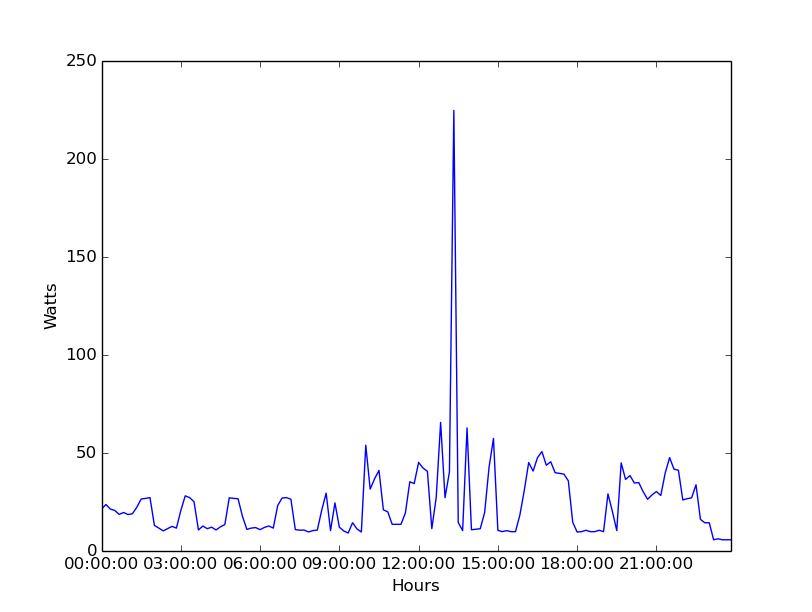
\includegraphics[width=1.0\textwidth]{img/only_interactive.png}
\caption[Difference]{\emph{\small Total consumption for interactive loads.}}
\label{interactiveLoads}
\end{figure}

\subsection{Results}
The total consumption trace of the household is illustrated in figure \ref{CompPlots}. The dashed blue line represents the original trace while the solid red line represents the trace with our scheduling algorithm least slack first (LSF). From the plot it is possible to see that the highest peak has been lowered from approximately 330 to 230 watts. Note that we already have a high peak in the interactive load. In the original trace without LSF, when both the fridge and the floor heater is powered  the peak is approximately 100 watts higher. With LSF on the other hand, the scheduler powers down both background loads at critical times. During the other hours the original and the LSF trace looks similar. There are just a few places where the solid line is significantly higher than the blue. This happens after the highest peak at 800 minutes. This happens since with LSF the execution of the background loads are postponed and will therefore yield in peaks later in time. These peaks however, never gets higher than the one caused by the interactive loads.

\begin{figure}[!ht]
\centering
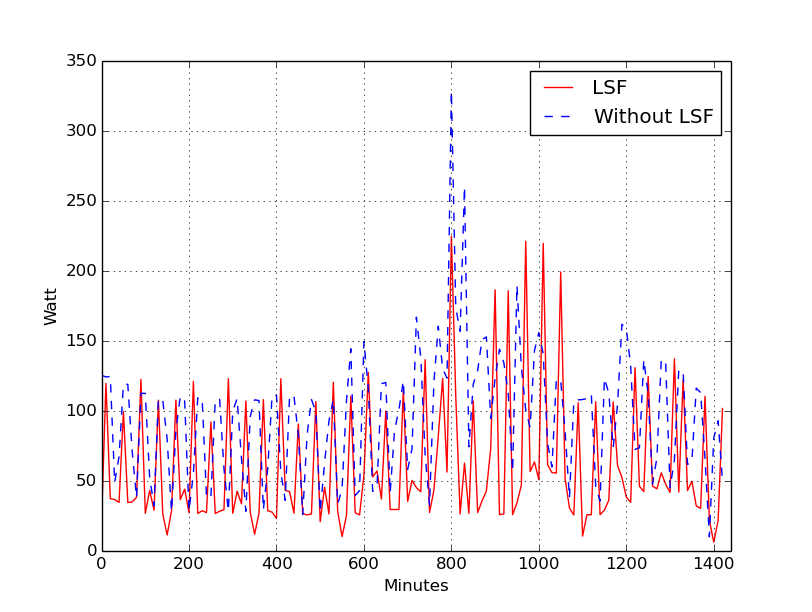
\includegraphics[width=1.0\textwidth]{img/comparizon.png}
\caption[Difference]{\emph{\small Power trace comparison during a 24-hour period.}}
\label{CompPlots}
\end{figure}

One of the issues with our test data is the large impact on the consumption caused by the floor heater. The floor heater frequently stands for more than 60 percent of the household's total consumption when active. This makes the consumption trace relatively pointed. Every time the floor heater is powered up, a spike in the consumption is noticed. A test set with more interactive loads and more background loads to control might help smoothing out the curve and yield in an even better consumption trace. Although it is wanted to avoid the worst peaks, a completely flat consumption is easier for the power suppliers to handle.

\subsection{Challenges}
\label{sec:challenges}
In this section we describe some of the challenges that we have faced. The challenges are related to the implementation of the system as well as the general idea itself.

\subsubsection{Third-party Library}
As we mentioned earlier we have used \emph{Plugwise} to implement this system. As there exists several other similar products we recommend using a product which has an open API. Since \emph{Plugwise} only offers a Windows based software with limited functions we had to program our own. We also wanted to prove that the solution easily can run on a Raspberry Pi, so we had to develop our own software for Debian/Linux operating system. Luckily, we found a third-party library for Python which we used \cite{hadaraplugwise}. The library turned out to have a couple of bugs which made it harder to use.

\subsubsection{Limitation of Test-data}
One of the biggest challenges is to find applicable test data. One or several real households need to be monitored with high granularity in order to observe how well the algorithm copes with sudden changes in the demand. Our test data is limited to one home during 24 hours and there are only a few devices that are being monitored. Furthermore, we only have the capability to control two background loads. Therefore, it is important to mention that the solution must be tested more thoroughly to evaluate the efficiency.

\subsubsection{The Threshold}
In order to have an efficient algorithm the threshold needs to be decided with great care. A threshold set too low will cause the scheduler to push the execution of the background loads on to the future, until the slack is zero and they are forced to run. This may lead to a forced execution in an inappropriate time. On the other hand, a threshold set too high would make the scheduler run all background loads simultaneously and then turn them all off when they reach their bound, yielding in a high peak followed by a low through.

\subsubsection{Infrastructure}
To get a system like this installed in a home today would require some effort. All background loads need to be equipped with smart plugs and sensors to be able to control and schedule them. Just to equip them with smart plugs is quite easy, but to equip them all with sensors as well is not as trivial. A better solution would be to use the already existing sensors in the appliances. This however, requires communication between the appliances and the scheduler. Even though more and more devices receive communication features, the so-called Internet of things, the vast majority of home appliances still cannot communicate.
\newpage
\section{Conclusion}
\label{sec:conclusion}
In this report we demonstrated that it is possible to lower the peak demand for a household without making the occupants change their habits. The components required are relatively cheap consisting of an off-the-shelf product coupled to our deployed software. Since the software is quite lightweight it is possible to implement and having it running from a small computer, e.g. a raspberry pi. The prototype in its current shape is probably more a proof of concept than an actual product. For normal consumers to apply a similar method in their homes, the components and software could be integrated into the home appliances and allowing the system to utilize the sensors and control switches that already exist in home appliances today. The scheduler could, for example, be placed inside the smart meter and no extra devices needs to be purchased. This approach could thereby be phased into people homes when they upgrade their equipment. The system could also be installed in new-built homes directly and thereby speed up the transition.

For this change to happen, the electricity pricing model needs to be changed. The electricity providers should not charge you only for how much power you consume, but also for peak usage. This would give consumers and also home appliance manufacturers an incentive to push for a change. This could help the electricity providers avoid peaks in the grid and thereby lower the greenhouse emissions while at the same time lead to lower cost of maintenance of the distribution grid.

\subsection{Future Work}
All algorithms that try to flatten peak demand make decisions without knowing what will happen next in the household. They do not know which devices that are currently active and for how long they will be so. If an algorithm could identify what devices are being used in each given time slot, it could make a more qualified guess on the change of future demand. For example, if the microwave is turned on, the algorithm knows the typical behaviour of a microwave and could therefore anticipate the future demand. Furthermore, if the stove is turned on, the algorithm might anticipate that food is about to be cooked in the household and that more kitchen appliances will be used in the near future and therefore take some action and prepare for that scenario. However, this idea has also its cost. For the scheduler to know which appliances that are being used it would need to have communication with all interactive loads as well as all the background loads. This would require all manufacturers of home appliances to include such communication. One other solution is to let the scheduler perform thorough analysis of the active loads and compare it with known consumption traces of home appliances to guess what appliances are active. A problem with this solution is that one appliance does not behave exactly as one of a similar model, or as it did yesterday. Microwave ovens, for example, comes in different sizes with different features. Some have a max power of 800 watts while some have 1000 watts. There is also possible for the user to select the power level each time the microwave oven is used. This means that each microwave oven may have numerous consumption traces which, furthermore, differentiates from a microwave oven from another brand and model. In order to keep track of all these traces, a quite large database would be required. Another challenge with this kind of analysis is that it is uncertain. The scheduler can only measure the total consumption of all active loads. There might be several different scenarios that yield in the same total consumption and the scheduler will have no way to differentiate these. The total consumption of the toaster and the microwave may for example be equal to the consumption of the stove.

Another interesting idea is to check the efficiency of the algorithm (LSF) when applied on a larger scale, not just one household but a whole neighbourhood or a smaller city. When applying the algorithm on a larger scale one must also deal with new issues like privacy, how households can communicate without violating the privacy of the occupants.
\newpage
\medskip
\printbibliography
\end{document}